\documentclass[10pt,a4paper]{article}
\usepackage[margin=2.2cm]{geometry}
\usepackage{fontspec}
\usepackage{kotex}
\setmainfont{Apple SD Gothic Neo}
\setsansfont{Apple SD Gothic Neo}
\usepackage{amsmath,amssymb}
\usepackage{graphicx}
\usepackage{booktabs}
\usepackage{caption}
\usepackage[dvipsnames]{xcolor}
\usepackage[colorlinks=true,linkcolor=MidnightBlue,citecolor=MidnightBlue,
            urlcolor=MidnightBlue]{hyperref}
\usepackage{titlesec}
\titleformat{\section}{\large\bfseries}{\thesection}{0.6em}{}
\captionsetup{font=small,labelfont=bf}
\setlength{\parskip}{0.35em}
\setlength{\parindent}{0pt}

\usepackage{mdframed}
\newmdenv[linewidth=0.4pt,linecolor=gray!60,backgroundcolor=gray!5,
          innertopmargin=6pt,innerbottommargin=6pt,skipabove=8pt,skipbelow=8pt]{claimbox}
\newcommand{\claim}[2]{\begin{claimbox}\textbf{주장.} #1\par\smallskip
  \textcolor{gray!70}{\textbf{반증 조건.} #2}\end{claimbox}}

\title{\bfseries 열두 번째 도메인의 문이 열렸다\\[2pt]
\large 합류 관문 통과 --- $12{,}674$ 편이 $864$ 개의 라벨이 되기까지}
\author{월드모델 실험실 · 노트 $835$}
\date{2026-08-07}
\begin{document}\maketitle

\section{한 줄}

다년 백필($2023$-$01$-$01{\sim}2026$-$08$-$01$ · $1{,}299$일 · 실패 $0.76\%$ ·
누적 역행 $0.06\%$)이 완주했고, 사전등록된 관문이 열렸다: \textbf{q$85 =
1{,}488$명 $\to$ 문턱 위 $897$편 · K$=21$ 라벨 성립 $97.1\%$($\geq 90\%$) ·
학습 $475$($\geq 300$) · 유보 $389$.} 취소 조건은 발화하지 않았다 ---
\textbf{KOBIS 는 판의 $12$번째 도메인 확정 경로에 들어섰다}(예상 판 지분
$\sim 10\%$ · 합류는 재기선).

\begin{figure}[t]\centering
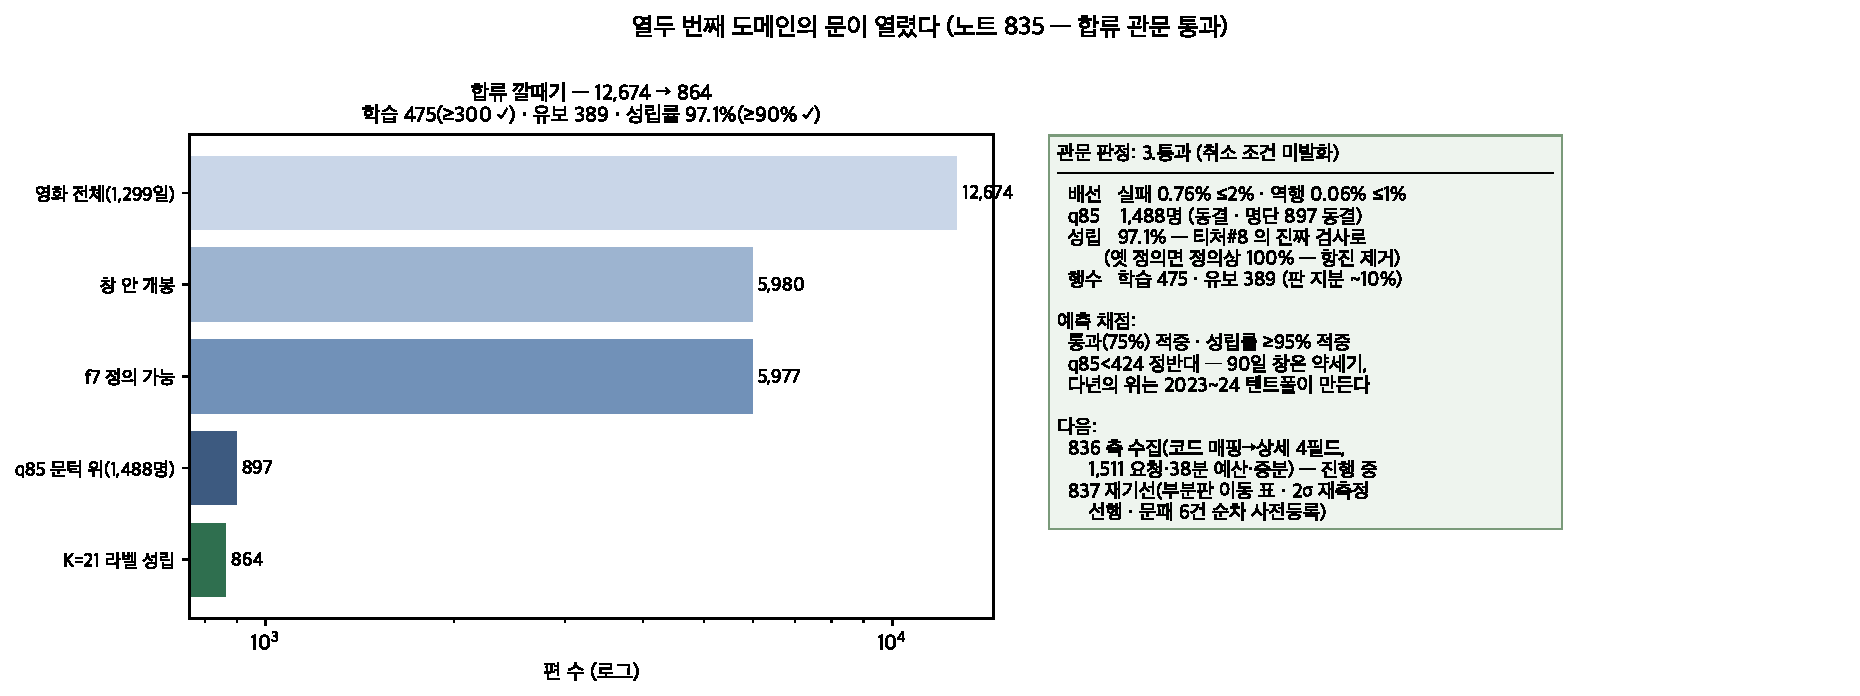
\includegraphics[width=0.97\textwidth]{figs/twelfth.pdf}
\caption{왼쪽: 합류 깔때기(로그). 오른쪽: 관문 판정과 다음 단계.}
\end{figure}

\section{두 티처가 이 관문을 정직하게 만들었다}

\claim{\textbf{성립률 $97.1\%$ 는 의미 있는 숫자다} --- 티처 \#$8$ 이 실행 전에
잡은 항진(above $\subseteq$ f$7$ 존재 $\subseteq$ 관측 존재 $\to$ 옛 정의로는
정의상 $100\%$)을 `마지막 관측 $\geq$ 개봉$+14$일'로 교체한 덕이다. 티처
\#$7$ 의 못 넷(q$85$ · K$=21$ · $2023$년 범위 · 전산망 밖 대조)도 전부 이
관문의 뼈다. q$85$ · 명단 $897$ · f$7$ 규칙은 값$+$코드로 동결했다(범위 쇼핑
금지).}
{예측 채점의 정직: 통과($75\%$)와 성립률($\geq 95\%$)은 적중, \textbf{q$85 <
424$ 는 정반대}($1{,}488$ --- $3.5$배 위). $90$일 창($2026$년 $5{\sim}8$월)은
성수기 부풀림이 아니라 \textbf{약세기}였고, 다년 분포의 위는 $2023{\sim}24$
텐트폴이 만든다 --- 계절 편향의 방향을 거꾸로 짚었다. 다음: $836$ 축
수집(코드 매핑 $\to$ 상세 $4$필드 · $1{,}511$ 요청 $38$분 예산 · 증분 저장 ---
진행 중) $\to$ $837$ \textbf{재기선}(부분판 이동 표 · $2\sigma$ 재측정 선행 ·
문패 $6$건 순차 사전등록). 판 $\rho$ $0.4689$ --- 이 숫자의 마지막 나날들이다.}

\end{document}
